\documentclass{beamer}
%\usepackage[russian]{babel}
\usepackage[utf8]{inputenc}
\usepackage{listings}
\usepackage{minted}


\usetheme[pageofpages=/,% String used between the current page and the
                         % total page count.
          bullet=circle,% Use circles instead of squares for bullets.
          titleline=true,% Show a line below the frame title.
          alternativetitlepage=false,% Use the fancy title page.
          watermarkheight=60px,% Height of the watermark.
          watermarkheightmult=4,% The watermark image is 4 times bigger
                                % than watermarkheight.
          ]{Torino}

\author{Presenting: Andrei Serebro\\
Supervisor: Dmitry Rykovanov (Geoscan)}
\title{Render-Based Power Pylon Positioning Using UAV Photos}
\institute{St Petersburg Academic University}
\date[b]{16 Mar 2017}
  
\definecolor{darkgreen}{rgb}{0,0.5,0}
\definecolor{dhscodebg}{rgb}{0.95,0.95,0.95}
\newminted[dhscode]{c++}{tabsize=4, fontsize=\footnotesize, frame=lines, framesep=5\fboxrule,framerule=1pt,
bgcolor=dhscodebg, rulecolor=\color{gray!40}}

\newcommand\hideit[1]{%
  \only<0| handout:1>{\mbox{}}%
  \invisible<0| handout:1>{#1}}

\AtBeginSection[]{
  \begin{frame}
  \vfill
  \centering
  \begin{beamercolorbox}[sep=8pt,center,shadow=true,rounded=true]{title}
    \usebeamerfont{title}\insertsectionhead\par%
  \end{beamercolorbox}
  \vfill
  \end{frame}
}



\begin{document}



\defverbatim[colored]\lstI{
\begin{lstlisting}[language=C++,basicstyle=\ttfamily,keywordstyle=\color{blue},commentstyle=\color{darkgreen}]
#define M1 1
#define M2 M1
#define M3 M2
...
int x = M3 + M3; // M3 expands two times
\end{lstlisting}
}

\defverbatim[colored]\lstRepeat{
\begin{lstlisting}[language=C++,basicstyle=\ttfamily,keywordstyle=\color{blue},commentstyle=\color{darkgreen},basicstyle=\small]
#define BOOST_PP_REPEAT_1_0(m, d)
#define BOOST_PP_REPEAT_1_1(m, d) m(2, 0, d)
#define BOOST_PP_REPEAT_1_2(m, d) \ 
           BOOST_PP_REPEAT_1_1(m, d) m(2, 1, d)
...
#define BOOST_PP_REPEAT_1_255(m, d) \
           BOOST_PP_REPEAT_1_254(m, d) m(2, 3, d)
\end{lstlisting}
}

\begin{frame}[t,plain]
\titlepage
\end{frame}

\begin{frame}[t, fragile]{Motivation}
Power lines inspection is important
\begin{itemize}
\item Power wire breakages
\item Insulator  breakages
\item \textbf{Power pylons inclinations}
\end{itemize}

Different solutions lead to different amount of manual labor\\
\begin{figure}
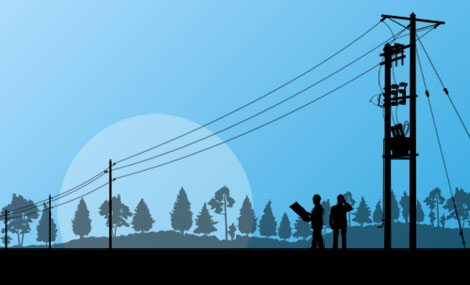
\includegraphics[scale=0.23]{inspection_people}
  \hspace{0.1cm}
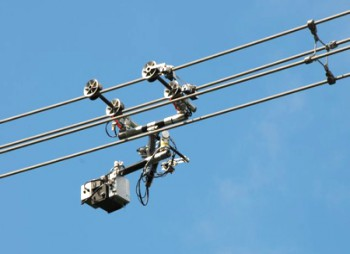
\includegraphics[scale=0.26]{inspection_robot}
  \hspace{0.1cm}
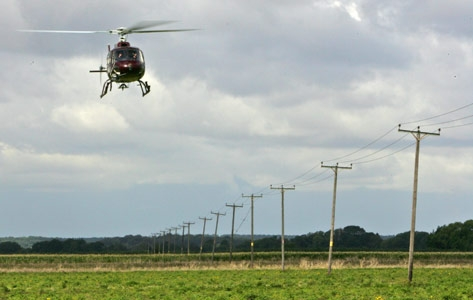
\includegraphics[scale=0.22]{inspection_helicopter}
\end{figure}
\end{frame}

\begin{frame}[t, fragile]{r/MildlyInteresting}
\begin{figure}
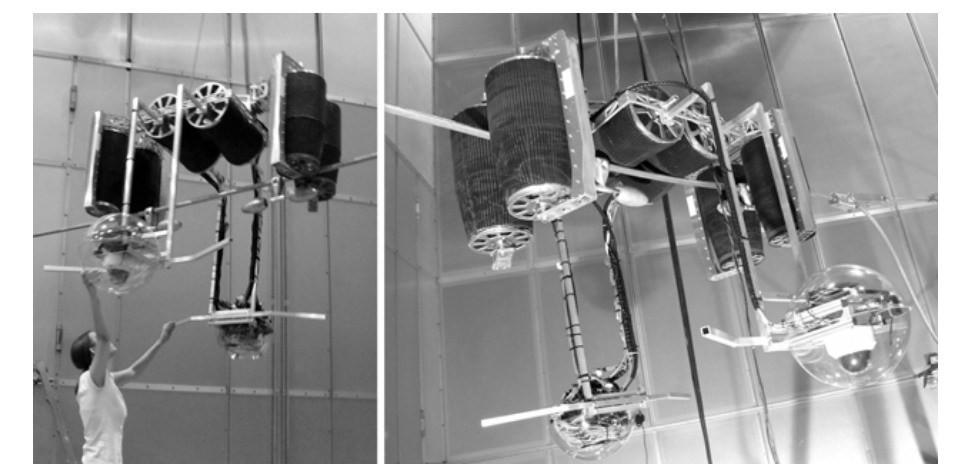
\includegraphics[scale=0.33]{canuimagine}
\end{figure}
\end{frame}

\begin{frame}[t, fragile]{Problem Statement}
Given:
\begin{itemize}
\item Set of images taken from UAV
\item Camera poses (e.g. extracted through any SFM pipeline)
\item 3D model of the scene, lacking power pylons
\item \lbrack Optional\rbrack  Calculated digital elevation model (DEM)
\end{itemize}
The goal is to:
\begin{itemize}
\item Estimate power pylon positions with sub-meter precision
\item Insert pylons into the model
\end{itemize}
\end{frame}

\section{Existing Solutions}

\begin{frame}[t, fragile]{Approaches Overview}
\begin{figure}
\centering
\includegraphics[width=0.8\linewidth]{approaches.png}
\label{fig:line3d_output}
\end{figure}
\end{frame}


\begin{frame}[t, fragile]{Approaches Overview: Photogrammetry + LiDAR}
Some studies in this area:
\begin{itemize}
\item [1] Gunho Sohn et al. "Automatic Powerline Scene Classification and Reconstruction Using Airborne LiDAR Data", 2012 
\item [2] Li et al. "A Model-Driven Approach for 3D Modeling of Pylon from Airborne LiDAR Data", 2015
\item [3] Bo Guo et al. "A Stochastic Geometry Method for Pylon
Reconstruction from Airborne LiDAR Data", 2016
\end{itemize}

LiDAR is typically heavy, we don't want to use it, yet the approaches from these papers are to be discussed

\end{frame}

\begin{frame}[t, fragile]{Key ideas of [1]}
\begin{itemize}
\item Split space into voxels 1.5 x 1.5 x 1.5 $\Rightarrow$ line voting, RANSAC
\item MRF to choose 3d lines representing power lines
\begin{itemize}
\item Line slope: PLs are almost horizontal
\item Height
\item Points \# in in-out cylinder (almost 0 for PL)
\item Line parallelism: PLs are parallel, pylons show random distribution
\end{itemize}
\item Pylon detection: RF classifier
\begin{itemize}
\item Maximum orientation variation (huge for pylons)
\item Orientation parallelism
\end{itemize}
\item Piecewise PL model growing
\end{itemize}
\end{frame}

\begin{frame}[t, fragile]{Key ideas of [2]}

\begin{itemize}
\item Pylon = set of parameterized parts (head, body, legs)
\item Detection via height variance map and density projection image
\item Head: SVM features = \{points height, front projection lengths\}
\item Position and orientation: contour planes; assume verticality
\item Body: frustum consisting of four planes (RANSAC)
\item Precision: said to be 0.03m in horizontal plane and 0.99$^\circ $
\end{itemize}
\begin{center}
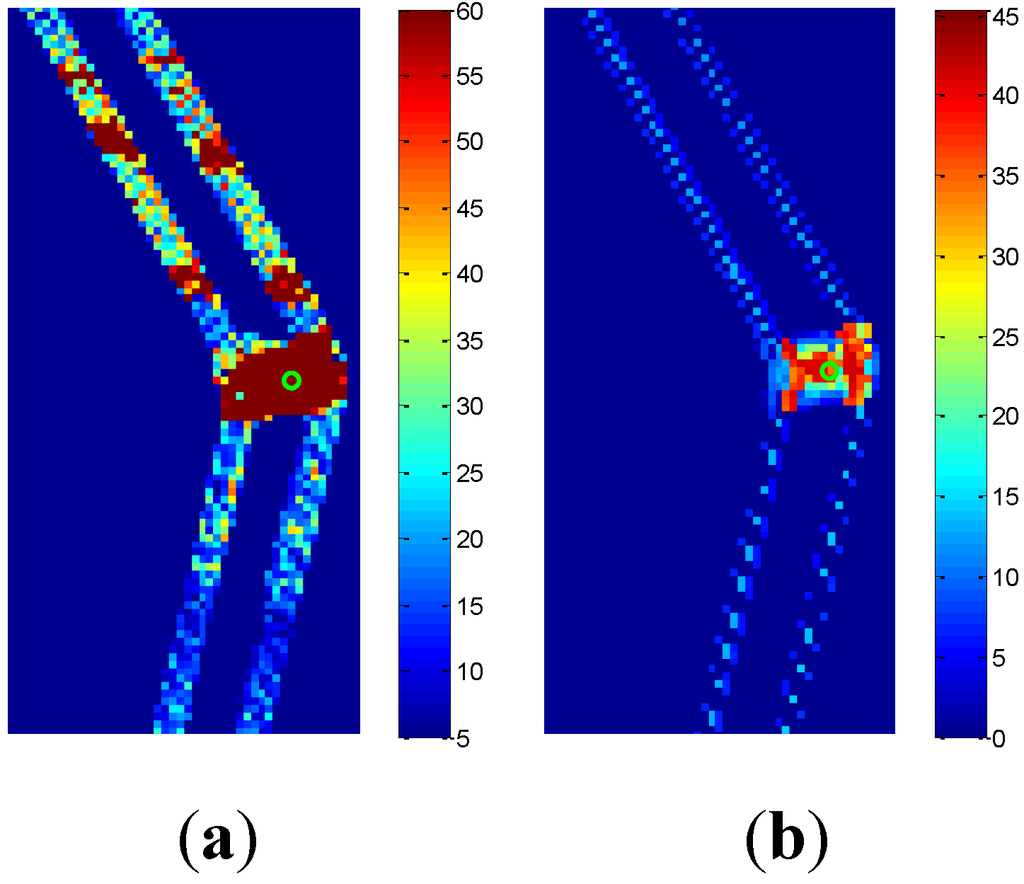
\includegraphics[width=0.3\linewidth]{model_based_lidar1}
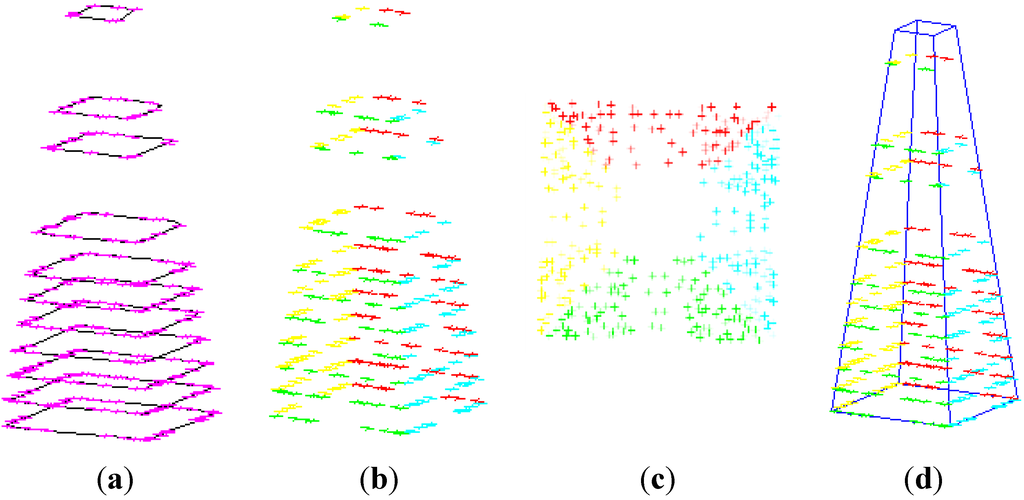
\includegraphics[width=0.5\linewidth]{model_based_lidar3}
\end{center}

\begin{flushright}
\small{$^*$Pictures from original work}
\end{flushright}
\end{frame}

\begin{frame}[t, fragile]{Key ideas of [3]}
\begin{itemize}
\item Again, model-based approach
\item JointBoost classifier to segment point cloud into pylons, wires, ground etc.
\item Graph-cut to eliminate outliers (pylons=foreground / rest=background)
\item Optimization problem: target combines distance from cloud to model and from model key points to cloud using MCMC
\item Precision: said to be 0.37m
\end{itemize}
\end{frame}

\begin{frame}[t, fragile]{Approaches Overview: Pure Photogrammetry}

Disclaimer: SIFT + PMVS perform poorly: wiry structures are thin and textureless $\Rightarrow$ small amount of feature points 

\begin{itemize}
\item [4] M. Hofer, "Line-based 3D Reconstruction of Wiry Objects", 2013.
\item [4'] M. Hofer, "Efficient 3D scene abstraction using line segments", 2016
\item [5] A. Correa, "UAV vision system: Application in electric line following and 3D reconstruction of associated terrain", 2017
\item [6] B. Morarjee, "Using Multiple View Geometry for Transmission Tower Reconstruction", 2016

\item [7] O. Araar, N. Aouf, "Power pylon detection and monocular depth
estimation from inspection UAVs", 2015
\end{itemize}
\end{frame}

\begin{frame}[t, fragile]{Key ideas of [4]}
Line3D is an open source C++ library which reconstructs 3d line segments form the set of images, developed as PhD by Manuel Hofer
\begin{itemize}

\item Supports many SFM frameworks
\item Can be used either standalone or as a library
\item Key ideas: 
\begin{itemize}
\item 2d LSD on each image
\item large set of 3d matching hypotheses (epipolar matching)
\item color histogram similarity
\item collinearity
\end{itemize}
\end{itemize}
Unfortunately, very poor results when wiry object is far and the number of photos is small
\end{frame}

\begin{frame}[t, fragile]{Line3D Timing}
Data taken from [4], time is in minutes
\begin{figure}
\centering
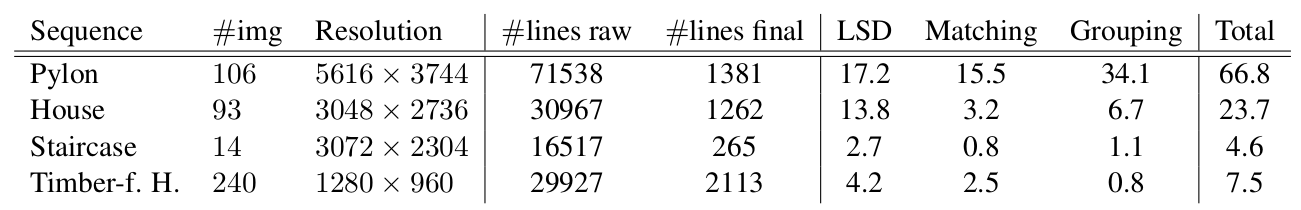
\includegraphics[scale=0.25]{line3dtime}
\end{figure}

[4'] improves runtime significantly (up to 8 times)
\end{frame}


\begin{frame}[t, fragile]{Line3D output sample}
Maybe, this can be used...
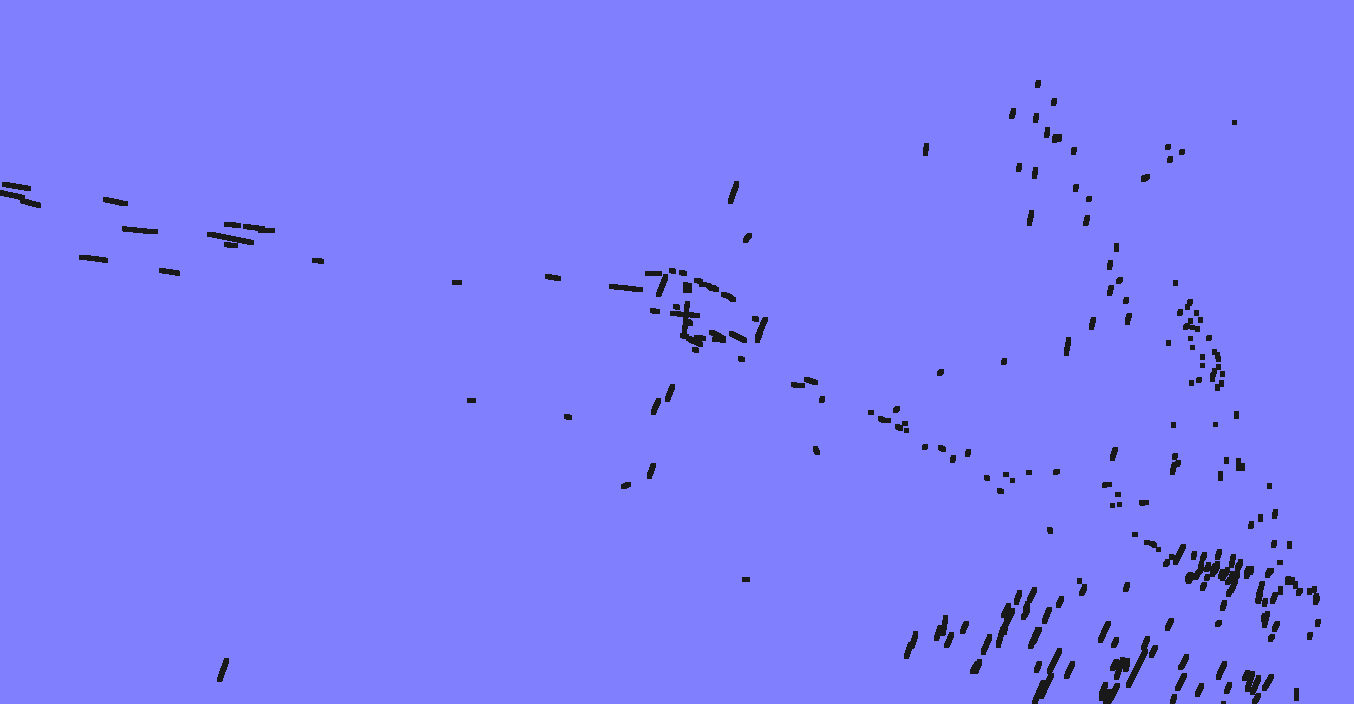
\includegraphics[width=1\linewidth]{line3d_output}
\end{frame}



\begin{frame}[t, fragile]{Key ideas of [5]}
\begin{itemize}
\item [1] Power line detection
\item [2] \textbf{Power towers detection}
\item [3] UAV visual-based navigation
\item [4] \textbf{3D reconstruction of electrical infrastructure}
\end{itemize}

\begin{itemize}
\item Custom line detection algorithm Circle Based Search
\begin{itemize}
\item Said to be faster than Hough/LSD when dealing with long lines
\item Not so precise with short lines; but it is feature in case of wire detection
\end{itemize}
\item Pylon detection through SVM
\begin{itemize}
\item ORB descriptor for features
\item ROI is splitted into cells and for each cell decision is made
\item Time per image (640 x 480) is 25 ms 
\end{itemize}
\end{itemize}
\end{frame}

\begin{frame}[t, fragile]{Key ideas of [6]}
M. Hofer's epigon: uses Line3d

\begin{figure}
\centering
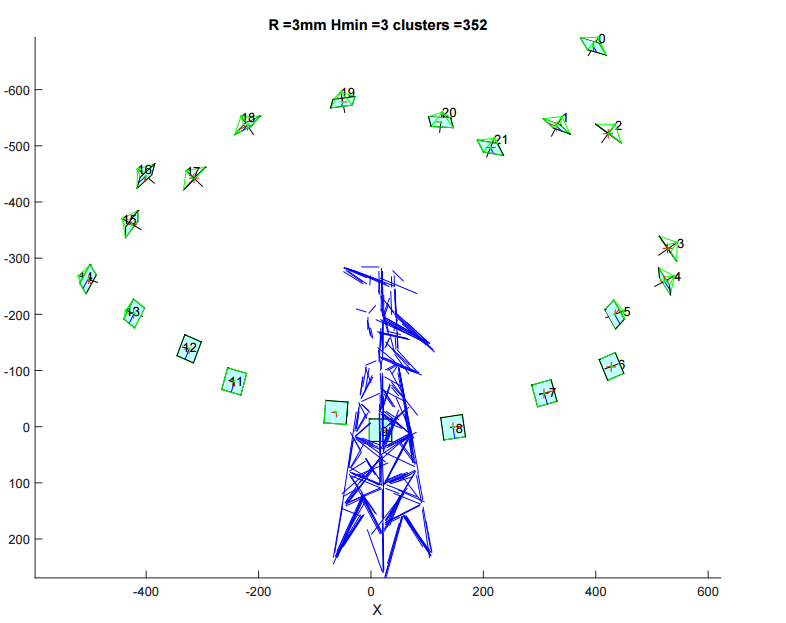
\includegraphics[scale=0.25]{morrarjee}
\end{figure}
\end{frame}

\begin{frame}[t, fragile]{Interesting idea of [7]}
\begin{figure}
\centering
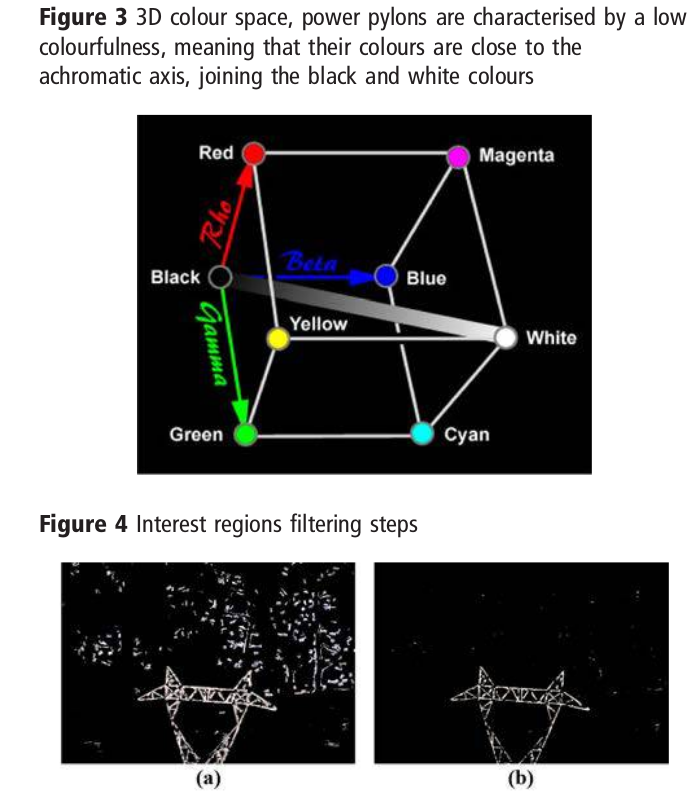
\includegraphics[scale=0.23]{colorful}
\end{figure}
\end{frame}

\section{Suggested Approach}

\begin{frame}[t, fragile]{Overview}
\begin{figure}
\centering
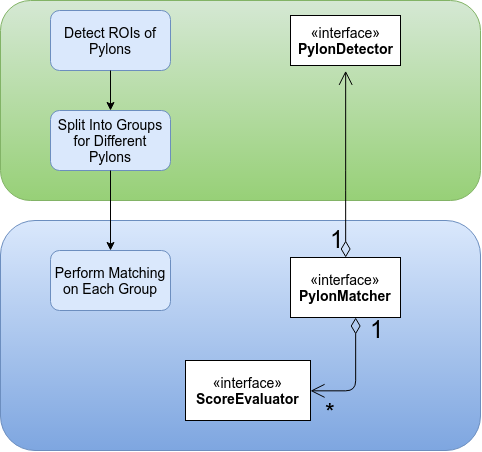
\includegraphics[scale=0.5]{Pipeline}
\end{figure}
\end{frame}

\begin{frame}[t, fragile]{Pylon Detection}
Current simple (yet working in non-urban scenes) strategy:
\begin{itemize}
\item Find power wires
\item Wires intersection $\Rightarrow$ pylon
\item Knowing pylon height and having DEM, evaluate 3d point and project on neighbor images
\end{itemize}
Interestingly, never seen it used anywhere
\begin{itemize}
\item Probably due to inefficiency: $\approx$ 3 seconds per photo (6000x4000)
\item Probably due to problems in urban areas
\end{itemize}
\end{frame}



\begin{frame}[t, fragile]{Feasibility}
\begin{figure}
\centering
\includegraphics[scale=0.13]{dirhard}
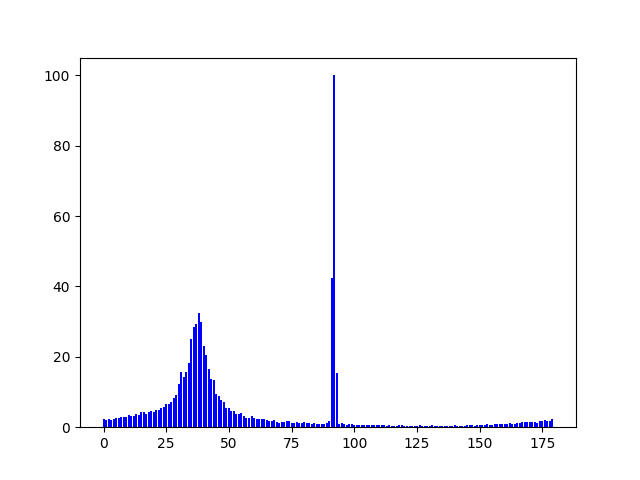
\includegraphics[scale=0.4]{dirhisthard}
\end{figure}
\end{frame}



\begin{frame}[t, fragile]{Pylon Detection}
\begin{figure}
\centering
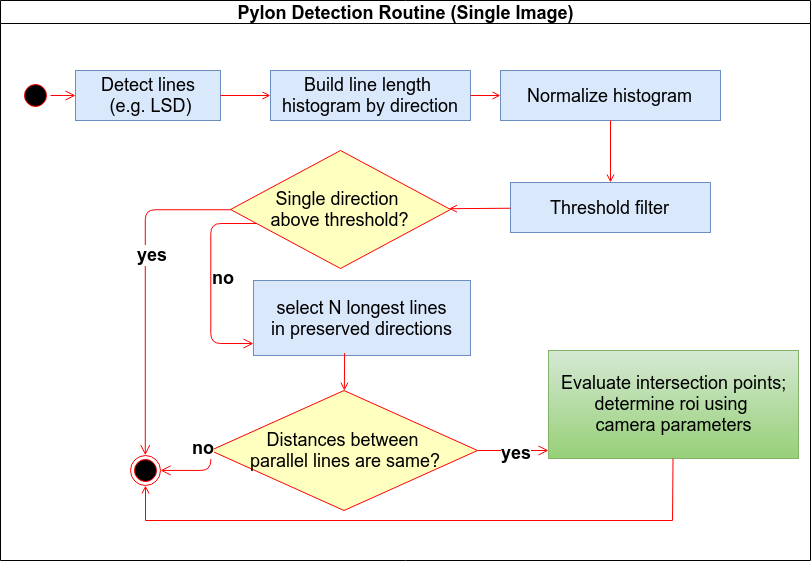
\includegraphics[scale=0.33]{DetectionSimple}
\end{figure}
\end{frame}

\begin{frame}[t, fragile]{Possible Pylon Detection Enhancements}
\begin{itemize}
\item Maybe use CBS algorithm proposed in \lbrack 5\rbrack
\item Use some ML for efficiency and robustness
\begin{itemize} 
\item SVM or neural networks
\end{itemize}
\item Search corners instead of lines
\end{itemize}
\end{frame}

\begin{frame}[t, fragile]{Detection Results Example}
\begin{figure}
\centering
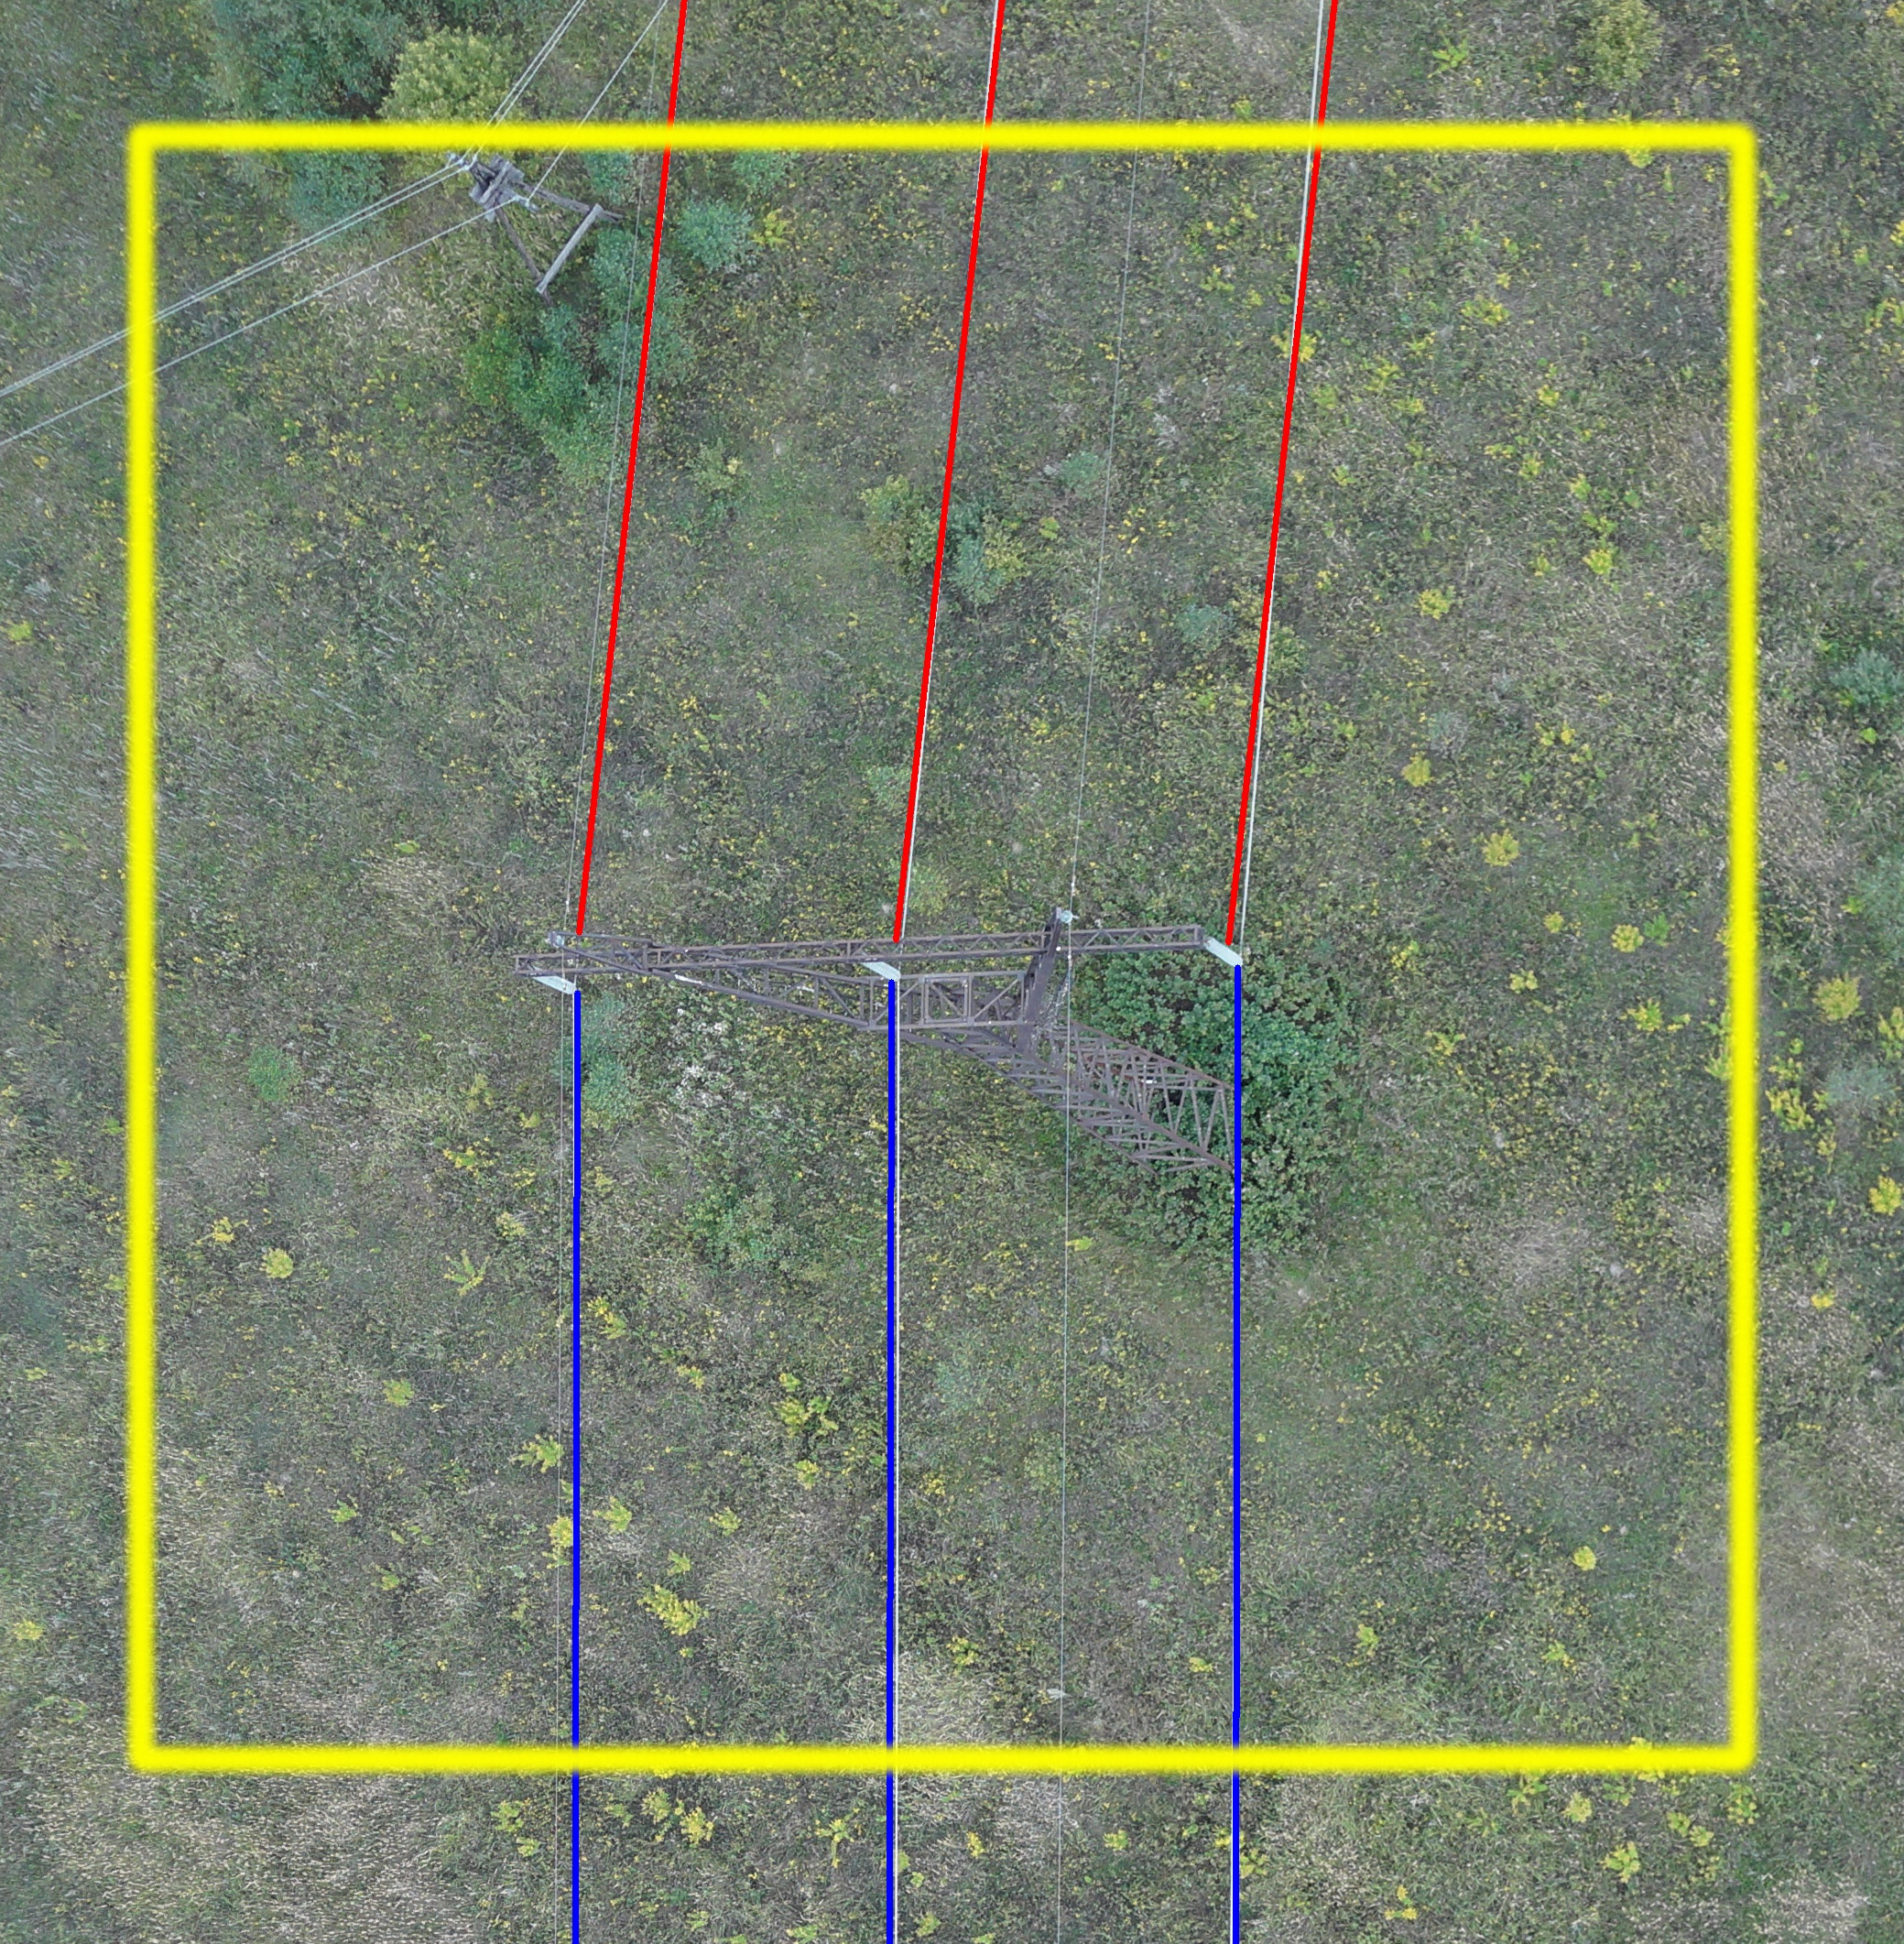
\includegraphics[scale=0.045]{intersection1}
\end{figure}
\end{frame}

\begin{frame}[t, fragile]{Detection Results Example}
\begin{figure}
\centering
\includegraphics[scale=0.045]{intersection2}
\end{figure}
\end{frame}


\begin{frame}[t, fragile]{Extracted ROI segments}
\begin{figure}
\centering
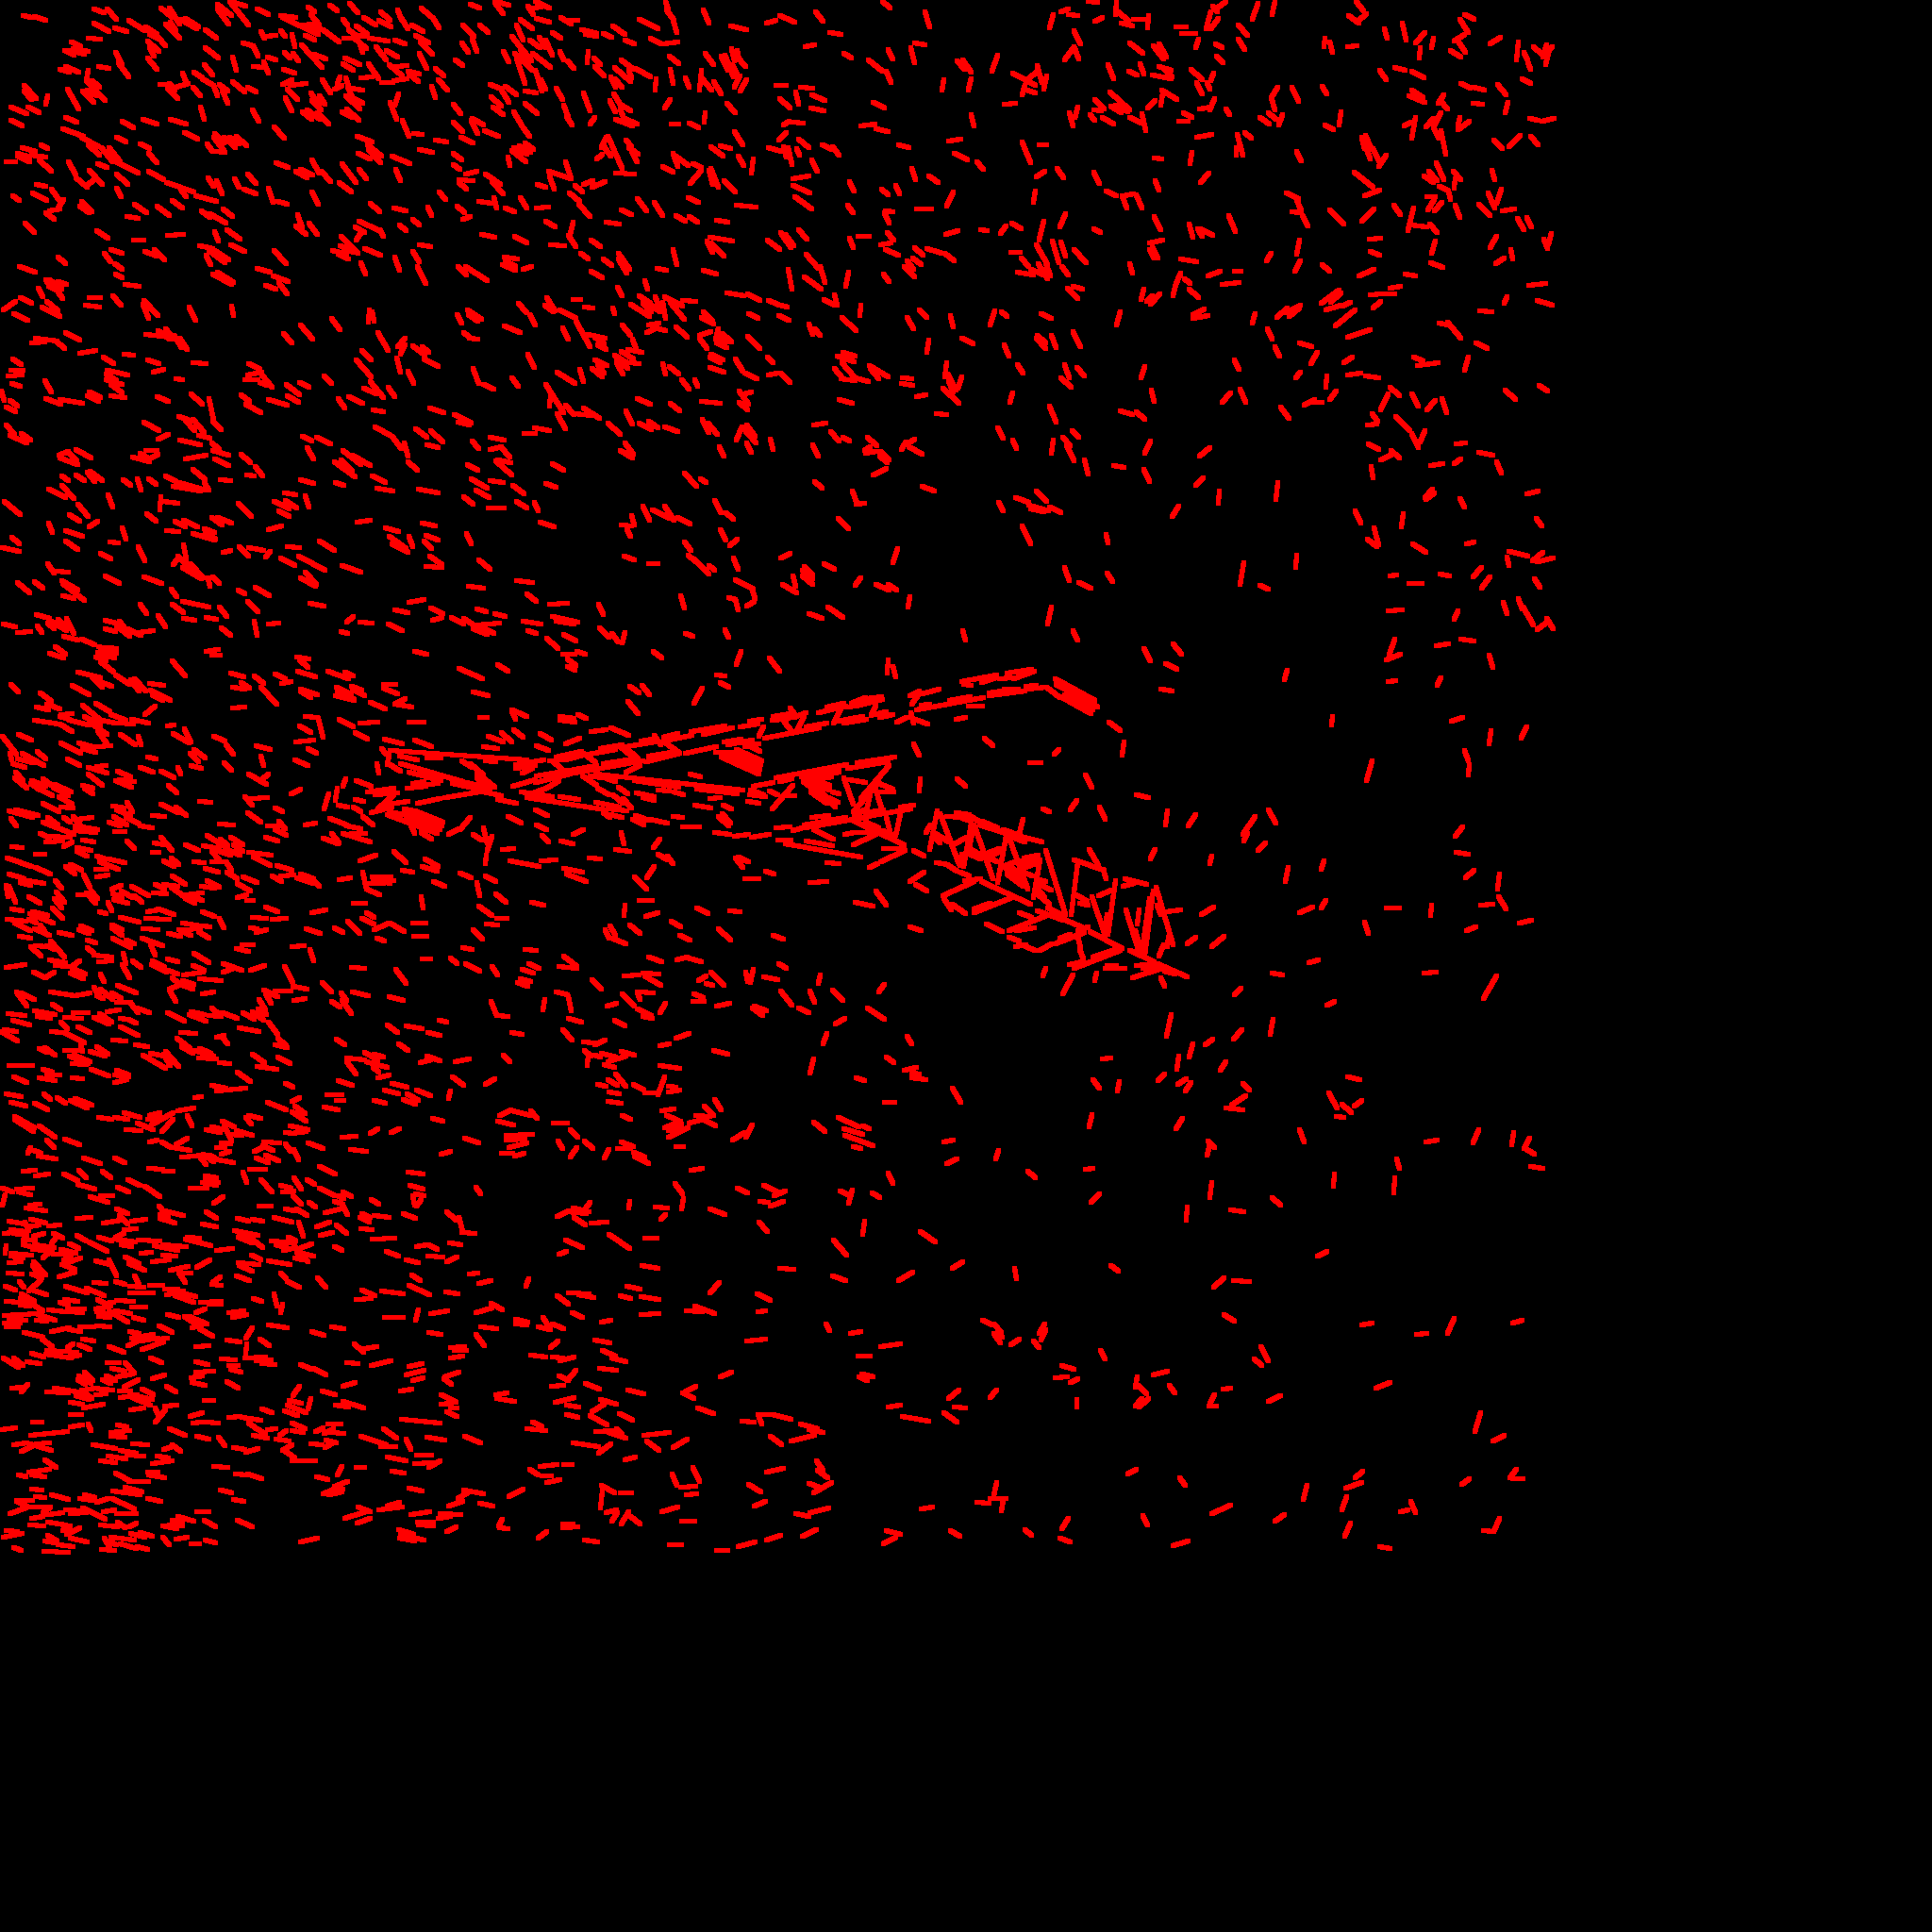
\includegraphics[scale=0.11]{roi}
\end{figure}
\end{frame}

\begin{frame}[t, fragile]{Pylon Matching}
Currently 2 exhaustive search solutions are proposed
\begin{itemize} 
\item[1] Render solid model
\begin{itemize} 
\item Score = \# of pixels from reference, overlapping with rendered model
\end{itemize}
\item[2] Render wiry model
\begin{itemize} 
\item Split image into grid (e.g 10 x 10 pix)
\item In each cell accumulate number of lines intersecting it in different directions
\item Use this information as features for any classifier
\end{itemize}
\end{itemize}

Open problem: need somehow combine estimations gained from several photos
\begin{itemize} 
\item Different reliability according to lines number, clamped ROI size
\item Probably something smarter than regression 
\end{itemize}
\end{frame}

\begin{frame}[t, fragile]{Solid Model Matching}
\begin{figure}
\centering
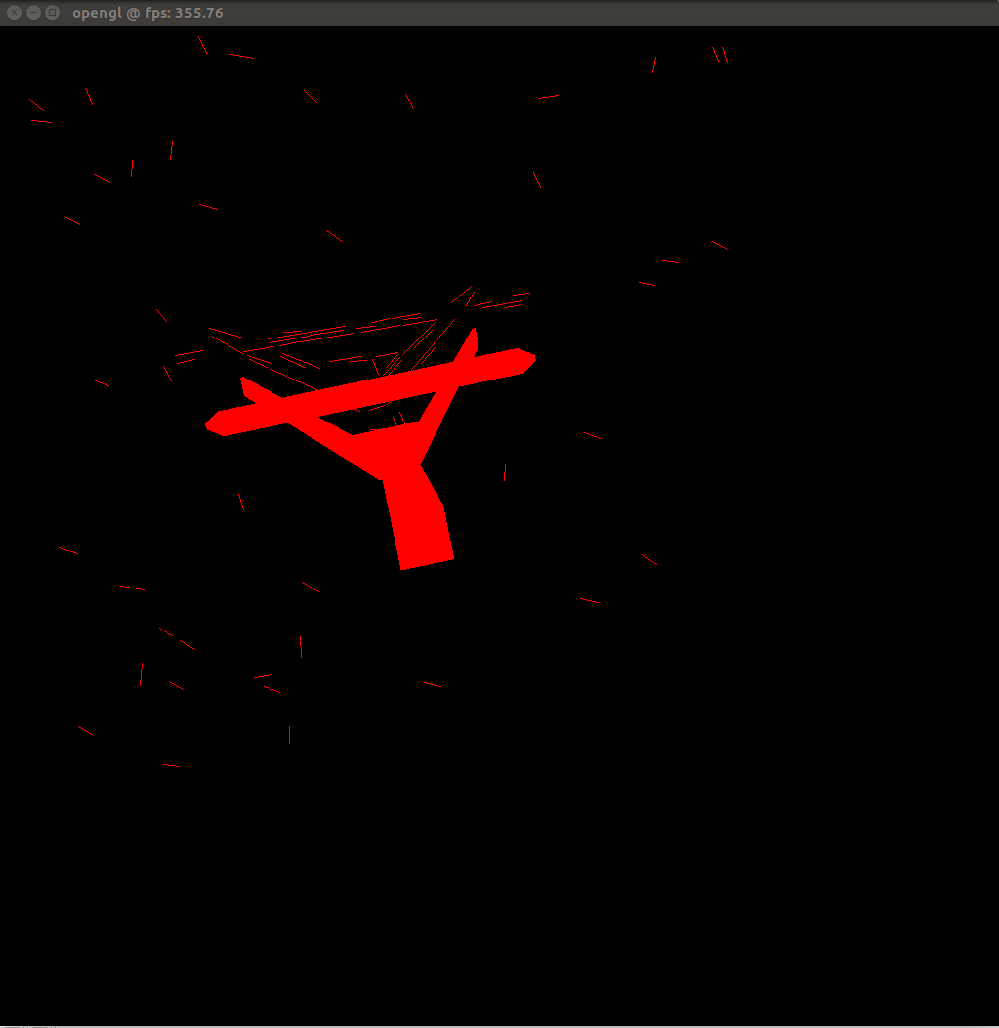
\includegraphics[scale=0.18]{render}
\end{figure}
\end{frame}

\begin{frame}[t, fragile]{Solid Model Matching Problems}
\begin{itemize}
\item Need to filter non-pylon lines carefully (currently by length)
\begin{itemize}
\item Maybe use graph-cut approach with color/orientation/length constraints as seed
\end{itemize}
\item Height estimation (why?)
\begin{itemize}
\item Currently, height is taken from DEM (not good at all!)
\end{itemize}
\item Slow: about 600-700 fps on nvidia 840M, about 1000 fps on gtx 1080
\begin{itemize}
\item Search space: 180 directions, $\pm 4$ meters in x, y with precision 0.1 gives us 1152000 variants $\Rightarrow$ 20 minutes per photo! Insane
\item Yet no evidence wiry model will be faster: exhaustive search should be replaced with something smarter
\item Trivial idea: score substantially different positions, then perform exhaustive search near maxima
\item Use Line3D output as additional ground truth
\end{itemize}
\end{itemize}
\end{frame}

\begin{frame}[t, fragile]{Wiry Model Matching}
\begin{itemize}
\item Perform render and grid intersection via CUDA
\item Parallelism: one thread per segment
\item Bresenham's line algorithm for line-grid intersection
\item Currently fps is similar to solid matching approach, but shared memory and improved parallelism can be considered
\item Score evaluation
\begin{itemize}
\item Naive: remember non-zero bins, score = percentage of these bins which are populated during model rendering [Currently implemented]
\item Convolute result with gaussian kernel: i.e. we choose two kernels - 2D kernel for spatial smoothing and 1D kernel for angle smoothing, so that rendered segment contributes to several bins simultaneously with different weights
\end{itemize}
\end{itemize}
Profit: no problems with height estimation
\end{frame}


\begin{frame}[fragile]{Thank You for Your Attention}

\begin{center}
\Huge Q \& A
\end{center}
\end{frame}


\end{document}

